\documentclass[11pt,a4paper,titlepage]{report}
\usepackage[utf8]{inputenc}
\usepackage[norsk]{babel}
\usepackage[parfill]{parskip}
\usepackage{wrapfig}
%\usepackage[htt]{hyphenat}
\usepackage{graphicx}
\usepackage{hyperref}
\usepackage{tabulary}
\usepackage{array}
\hyphenation{Elasticsearch}
\renewcommand{\arraystretch}{1.5}
\author{Gruppe19}
\title{Forprosjektrapport}
\begin{document}
\maketitle
\tableofcontents

\newcommand{\mw}{\emph{Making Waves}}
\newcommand{\es}{\emph{Elasticsearch}}
\newcommand{\rb}{\emph{Redd Barna}}
\newcommand{\cs}{C\nolinebreak\hspace{-.05em}\raisebox{.6ex}{\scriptsize\bf \#}}

\chapter{Presentasjon}
\vspace{-1.5cm}
\begin{flushleft}
\renewcommand{\arraystretch}{1.5}
\begin{tabular}[ht]{@{}lp{100mm}@{}}
\textbf{Oppdragsgiver} & 
\begin{wrapfigure}{r}{0.25\textwidth}
\vspace{-0.75cm}
\hspace{-2.5cm}

\includegraphics[scale=0.15, keepaspectratio]{./img/presentasjon/mw_logo.png}
\end{wrapfigure}
\vspace{-0.25cm}
\href{http://www.makingwaves.no/}{Making Waves} (MW) \newline Kristian IVs gate 13 \newline 0164 Oslo \newline +47 22 206 020 \newline \href{mailto:post@makingwaves.com}{post@makingwaves.com} \\
\textbf{Prosjekteier} & 
\begin{wrapfigure}{r}{0.25\textwidth}
\vspace{-0.75cm}
\hspace{-2.5cm}

\includegraphics[scale=0.075, keepaspectratio]{./img/presentasjon/rb_logo.jpg}
\end{wrapfigure}
\vspace{-0.3cm}
\href{http://www.reddbarna.no/}{Redd Barna} \\
\textbf{Prosjekttittel} & Redd Barna \\ 
\textbf{Oppgave} & - \\ 
\textbf{Periode} & 04.01.2016 - 28.05.2016 \\ 
\textbf{Gruppenummer} & 19 \\ 
\textbf{Gruppemedlemmer} & Espen Bjorøy Zaal - s198599 \newline Lukas David Larsed - s198569 \newline Henrik Fischer Bjelland - s198570\newline Simen Flatby - s198577 \\ 
\textbf{Gruppeleder} & Espen Bjorøy Zaal \\ 
\textbf{Intern veileder} & Thor E. Hasle \\ 
\textbf{Eksterne veiledere} & Marius Slette Johansen \newline Manager for Portals, Commerce and Data Analysis \newline \href{mailto:marius.johansen@makingwaves.no}{marius.johansen@makingwaves.no} \newline +47 982 48 333 \newline \newline Kaare Øystein Trædal \newline Client Director \newline \href{mailto:kaare.tradal@makingwaves.com}{kaare.tradal@makingwaves.com} \newline +47 970 08 137 \\
\textbf{Prosjektside} & \url{http://cerveceroscodigo.org/} \\
\end{tabular} 
\end{flushleft}

\section{Oppdragsgiver}
Making Waves er eksperter på digital tjenesteutvikling og innovasjon. Hos Making Waves finner du rådgivning, design, teknologi, innholdsproduksjon og drift under samme tak. Making Waves er en digital innovasjonspartner for mange av Nordens største merkevarer og offentlige virksomheter.

Making Waves ønsker å inkludere studentene i sine prosjekter gjennom å gi en oppgave som er løsbar på normert tid, og som vil utfordre og lære studentene til å bruke sin kunnskap og lære mer om utvikling, prosjekt og teknologi.

Oppgaven er tenkt å løse en utfordring i et prosjekt hvor det er muligheter for å gjøre utvidelser eller nyutvikling av en tjeneste tilknyttet Redd Barna.

Making Waves vil stille med faglig veiledning i prosjektet. Studentene kan forvente å jobbe sammen med Making Waves sine eksperter på .NET og søk.

\section{Oppgave}
Gjennom informasjon studentene har fått tilgang til har det kommet frem at et av Redd Barnas største mål for 2016 er å skape bedre relasjoner og lojalitet til sine eksisterende givere. Dette målet har opphav i informasjon som sier at om en giver har vært medlem i 6 måneder i strekk er sjansen for at han forblir giver livet ut særdeles stor.

For å nå dette målet har gruppen sammen med Making Waves og Redd Barna kommet frem til at det skal lages en personlig nettside eller en "Min side". Oppgaven vil i korte trekk gå ut på å lage denne siden og alt som trengs for at den skal fungere som en selvstendig applikasjon.

Studentene vil få tilgang til en dump av det datasettet Redd Barna sitter på i form av medlemsregister, giverhistorikk og kundekommunikasjon. Denne dumpen kommer i CSV-format.

Moduler som vil være nødvendig for en slik applikasjon vil blant annet være:
\begin{itemize}
\item Import av data fra CSV til Elasticsearch
\item Front end i HTML og JavaScript
\item WebAPI i C\# eller Node.js
\item Dataaksesslag i C\# eller Node.js som aksesserer Elasticsearch
\end{itemize}

Om tiden skulle strekke til vil det også være aktuelt for gruppen å lage en administrasjonsside som ansatte i Redd Barna kan bruke til å se på statistikk.
\chapter{Problemstilling}
For at oppgaven med å lage en ``Min side'' skal kunne løses trenger gruppen tilgang til medlemsdata fra Redd Barna.

Redd Barna er nå i en fase hvor de velger seg et nytt CRM-system (Customer relationship management eller Kunderelasjonshåndtering). Dette valget skal være tatt i løpet av Februar, men for å slippe å vente på at dette systemet er oppe og går har gruppen sammen med oppdragsgiver bestemt at det tas en dump av medlemsdata fra deres gamle CRM-system slik at det er et avtalt datasett som gruppen kan forholde seg til. 

Datadumpen studentene får tilgang til vil inneholde medlemsregister, giverhistorikk og kundekommunikasjon. Denne dumpen kommer i CSV-format. Dette vil være utgangspunktet for hvilke data studentene har å jobbe med. Fordi Elasticsearch skal brukes til håndtering av data vil det være nødvendig å lage script som parser dataene til JSON og dytter de inn i Elasticsearch.
\chapter{Mål og avgrensninger}
\section{Mål}
Bachelorprosjektet gir gruppen en utmerket mulighet for å jobbe sammen med erfarne folk i arbeidslivet. Making Waves har vært veldig behjelpelig og imøtekommende for å legge til rette for gruppen, slik at det daglige arbeidet skal foregå i Making Waves sine lokaler, sittende rett ved de som er involvert i prosjektet til Redd Barna.

Gruppens konkrete mål er:
\begin{itemize}
\item Lære så mye om det tekniske innen faget som mulig.
\item Lære av de erfarne fagfolkene i Making Waves, om hvordan teamarbeid, arbeidsprosesser og prosjektstyring foregår.
\item Utvikle gruppens evne til å analysere problemstillinger, lage kravspesifikasjon og fremlegge forslag til løsninger og utbedringer i forhold til dagens situasjon.
\item Gjøre et så godt arbeid at Making Waves ønsker å ta i bruk hele eller deler av koden som er produsert.
\end{itemize}

På generell basis ønsker gruppen å leve opp til gruppens egne, høye forventninger. Gruppens medlemmer har hatt gode resultater gjennom hele studiet og Bachelorprosjektet skal være kronen på verket.

\section{Avgrensninger}

\chapter{Arbeidsmetodikk}
\section{Metode}
To arbeidsmetoder ble vurdert i forkant av prosjektet, Scrum og Kanban.

I Scrum begynner man med å definere user stories eller brukerhistorier på formen ``Som (rolle) ønsker jeg (funksjonalitet), sånn at (fordel)''. Disse brukerhistoriene blir gjort om til kort i en product backlog. Videre bestemmer eieren av prosjektet hvilke kort som er viktigst og prioriterer kortene i rekkefølge deretter. Utviklere estimerer hvor lang tid det tar å utføre oppgaven på et kort i timer eller dager. Ut i fra rekkefølgen på kortene og hvor lang tid som er estimert bestemmes hvor mange kort som skal tas med i en iterasjon eller sprint (for eksempel en uke eller to uker). Når en sprint er ferdig skal alle oppgavene være gjort og man skal kunne levere gjeldende funksjonalitet til kunden. En person i teamet får rollen Scrum-master. Scrum-masters oppgave er å legge til rette for at alle får gjort det de skal samt å administrere product backlog'en sammen med produkteieren.

I Kanban har man en product backlog med kort på samme måte som i Scrum, men i steden for å jobbe i sprinter setter man opp en tavle med kolonner som representerer hvilket stadie hver oppgave er i. Eksempler på kolonner kan være:
\begin{itemize}
\item To do
\item In progress
\item In testing
\item Deployed
\end{itemize}
I en kolonne kan det maks være et avtalt antall kort av gangen, for eksempel 4. Dette forhindrer at en oppgave som er påbegynt ikke blir ferdigstilt innenfor rimelig tid.

Gruppen fant sammen med oppdragsgiver ut at Scrum vil føre til i overkant mye prosjektstyring når vi bare er fire stykker i gruppen og har derfor valgt å gå for Kanban. Gruppen mener dette vil gi en smidig utviklingsprosess med god oversikt over hva som må gjøres til en hver tid.

\section{Roller}
For at det skal være klart hvem som har ansvar for hva har gruppen deffinert noen ansvarsområder:
\begin{flushleft}
\renewcommand{\arraystretch}{1.5}
\begin{tabular}[ht]{@{}ll@{}}
\textbf{Gruppeleder} & Espen Bjorøy Zaal \\
\textbf{\LaTeX} & Lukas David Larsed \\
\textbf{Kommunikasjon med oppdragsgiver} & Henrik Fischer Bjelland \\
\textbf{Kommunikasjon med forskningsprosjektsleder} & Espen Bjorøy Zaal \\
\textbf{Versjonskontroll (Git og integrasjon)} & Lukas David Larsed \\
\textbf{Internkommunikasjon (Slack og integrasjon)} & Simen Flatby \\
\end{tabular} 
\end{flushleft}
Ved eventuelle diskusjoner hvor gruppens medlemmer ikke kommer til flerstemt enighet vil gruppeleders stemme telle dobbelt.

\section{Prosjektstyring}
\begin{wrapfigure}{r}{0.5\textwidth}
\vspace{-0.5cm}
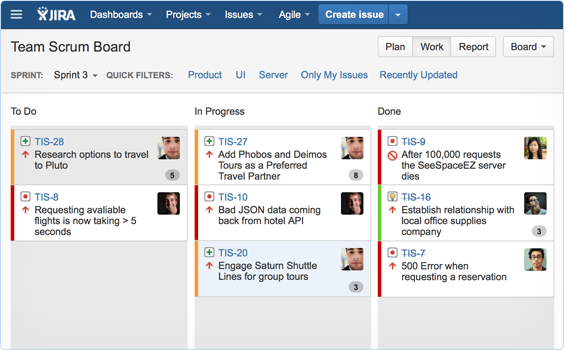
\includegraphics[scale=0.5, keepaspectratio]{./img/arbeidsmetodikk/jira_kanban.png}
\end{wrapfigure}
Til styring av prosjektet har vi valgt å bruke \href{https://www.atlassian.com/software/jira}{Jira}. Jira egner seg godt til bruk med Kanban, og vil hjelpe oss å administrere arbeidsoppgavene våre. Jira har en rekke integrasjoner, og vi vil blant annet benytte oss av GitHub-integrasjonen for å lage koblinger mellom Kanban-kort i Jira og GitHub-issues.

\chapter{Løsninger}
\section{Teknologier}
\section{Moduler}

\chapter{Fremdriftsplan}

Fremdriftsplanen er kun tentativ og kommer sannsynlig å endres under prosjektets gang. Fremdriftsplanen er satt opp i form av \textit{fase} struktur med hensyn til preliminær planleging. Etter at prosjektet har startet kommer man til å overgå til smidig metodikk. 
\\

\begin{center}
\makebox[\textwidth][c]{  
\begin{tabulary}{1.2\textwidth}{|p{2cm}|p{2cm}|L|}
\hline
\textbf{Fase}	&	 \textbf{Periode}	&	\textbf{Beskrivelse}                                             \\	\hline

Oppstart 	& 	01.01.16 22.01.16	& 	
Oppstartfase der det er planlagt møter med veileder ved HiOA og MW. Innledende møter med kunde og brainstorming kring mulig løsning. Oppsett av prosjektverktøy, system for versjonskontroll, grupperoller og ansvarsområder. 
\\ \hline

Analyse og Planlegging		&	 25.01.16 12.02.16	&	Analyse av data og valg av teknologi. Møtevirksomhet med kunde (Redd Barna). Arkitektur og systemutvikling.
\\ \hline

Utvikling 1 &	15.02.16 12.03.16 	&	Deles inn i flere steg. Med testing mellom stegene. testing gjennomføres kontinuerlig.
\\ \hline

Utvikling 2	&	13.03.16 15.04.16 	&	Pågår frem til midten av april. Tilleggfunksjonalitet. Implementeringfase og integrasjon i eksisterende systemer.
\\ \hline

Påskeferie 	&	23.03.16 27.03.16	& Ferie. Fravær må påregnes. \\ \hline

Testing		&	16.04.16 01. 	&	Integrasjontesting og funksjonkontroll mot eksisterende systemer. \csh
\\ \hline

Rapport		&	07.05.16 27.05.16 	&	Tid reservert kun til arbeid med rapporten. Øvrige deler av rapporten skrives kontinuerlig under prosjektets gang. \\ \hline

\end{tabulary}  
}
\end{center}


\chapter{Noen eksempler på referanser}
Test av bilbiographi\cite{book:unixprog}.
Test referanse 2 \cite{book:unixprog2}.
Teksdlksadjf lka jdsf\footnote{Link til \href{www.vg.no}{Link til VG}}


\bibliographystyle{plain}
\bibliography{bibliography}
	




\end{document}